\chapter{文獻探討}
本章會將所有本論文參考到的技術一併介紹,首先會介紹歌聲分離領域中的傳統方法,雖然現今許多資訊科學解決的問題中,皆以深度神經網路解決,但仍必須建立在過往傳統的方法上,才能多面向的確認要解決的目標,並確立實驗的架構。再來,就是本篇論文主要著墨的地方—深度學習法,在現今技術越來越成熟,使用深度學習於歌曲人聲分離領域的做法不斷被提出,其中監督式學習(supervised learning)~\cite{kotsiantis2007supervised}在此領被廣泛的使用到,本論文在這些文獻中受到啟發,並改進既有 U-Net 的效能。

\section{傳統方法}
傳統的歌曲人聲分離方法需先將歌曲訊號進行短時傅立葉轉換(short-time Fourier transform)轉成頻譜,再透過分析頻譜進行人聲分離。

\subsection{重複結構擷取}
重複結構擷取 (repeating pattern extraction)~\cite{rafii2012repeating}。以伴奏軌為重複密集的結構前提,對應主唱軌的結構較為鬆散,以此假設,觀察其重複出現的頻譜結構,以此判斷頻譜中哪些部分屬於伴奏軌,剩餘部分為主唱軌。

\section{深度學習法}
本論文主要基於的 U-Net 架構(圖\ref{ronneberger1})為 Ronneberger~\cite{ronneberger2015u} 等人提出,用於分割生物醫學影像,並有很好的效果,本論文希望能使用此架構於歌聲分離的任務上。

\begin{figure}[htbp]
    \hfil
    \begin{minipage}[t]{1.0\textwidth}
        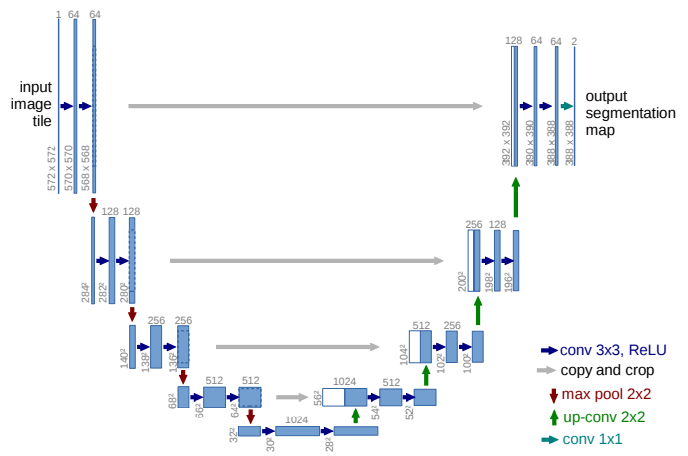
\includegraphics{./figures/chapter02_method/ronneberger1.png}
        \centering
        \caption {本論文主要研究的 U-Net 架構}
        \label{ronneberger1}
    \end{minipage}
    \hfil
\end{figure}

\subsection{濾波處理}
在頻譜域下的深度學習模型~\cite{hennequin2020spleeter,stoter20182018}通常會再採取濾波方法以增幅預測效果,且不增加太多預測時間(latency),首先定義下文會用到的符號。
\begin{itemize}
    \item $x(n)\in\mathbb{R}^2$ 表示混音軌(mixture stem)的時間序列
    \subitem $x(n)=s_{\textup{V}}{(n)} + s_{\textup{A}}{(n)} = \sum_{i\in\textup{I}}{s_i{(n)}}$
    \subitem $\textup{I} := \{\textup{V,A}\}$, $\textup{V}$: vocals主唱, $\textup{A}$: accompaniment伴奏
    \subitem $\hat{s_i}{(n)}$: 預測音軌的時間序列
    \item short-time Fourier transform (STFT) domain
    \subitem $X(m,f)\in\mathbb{C}^2$: 混音軌, $S_i(m,f)$: 來源分軌$_i$, $\hat{S_i}{(m,f)}$: 預測分軌$_i$
    \subitem $m$ 代表 frame;$f$ 代表 frequency bin
    \subitem $\vert\ast\vert$: STFT 的 magnitude, $\angle \ast$: STFT 的 phase
\end{itemize}

\subsubsection{Ratio Mask Filter}
% https://hal.inria.fr/hal-02293689/document
Ratio mask filtering 是一種直觀且簡單的作法,許多頻譜預測的方法~\cite{bao_abdulla_2018,stoter20182018}會再使用此,作為最後輸出訊號的遮罩,並且,可以此為基礎做另外衍伸。
\begin{equation*}
    \hat{S_i}{(m,f)} = \vert S_i(m,f)^E\vert (\sum_{j\in\textup{I}}\vert S_j(m,f)\vert^E)^{-1}X(m,f)
\end{equation*}
$E$ 代表 separation exponent,對於各種不同模型可以調整 ratio 以最佳化。
圖\ref{oracle_filtering1}與圖\ref{oracle_filtering2}\footnote{https://colab.research.google.com/drive/1Zo6iSPIi6SjOAL7wg8yzVWkS9mjLgjI-?usp=sharing}為實際 ratio mask 對主唱軌預測結果的遮罩與頻譜圖。

\begin{figure}[htbp]
    \hfil
    \begin{minipage}[t]{0.45\textwidth}
        \centering
        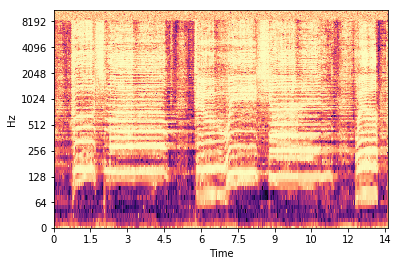
\includegraphics[width=\textwidth]{./figures/chapter02_method/oracle_filtering1.png}
        \caption {預測主唱軌的 ratio mask}
        \label{oracle_filtering1}
    \end{minipage}
    \begin{minipage}[t]{0.45\textwidth}
        \centering
        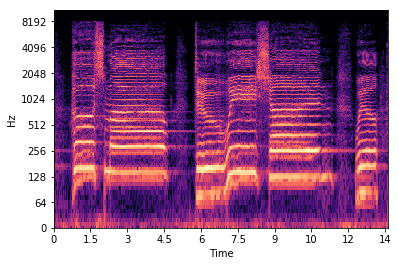
\includegraphics[width=\textwidth]{./figures/chapter02_method/oracle_filtering2.png}
        \caption {經過 ratio mask 濾過的頻譜}
        \label{oracle_filtering2}
    \end{minipage}
    \hfil
\end{figure}

\subsubsection{Wiener Filter}
Wiener filter 是一種古老的訊號學技術,由 Wiener~\cite{wiener1949extrapolation} 提出。在此,假設 $s_\textup{V}{(n)}$ 與 $s_\textup{A}{(n)}$ 為廣義平穩不相關隨機序列,其功率譜密度分別是 $P_{s_\textup{V}}{(\omega)}$ 與 $P_{s_\textup{A}}{(\omega)}$ ,功率譜相加的式子:
\begin{equation*}
    P_{x}{(\omega)} = P_{s_\textup{V}}{(\omega)} + P_{s_\textup{A}}{(\omega)}
\end{equation*}
% file:///C:/Users/hp/Documents/MIR_Lab/report/21Oct2020_report/21Oct2020_report.pdf
基於訊號的統計特性,為了最大化其中一個訊號 $s_i{(n)}$,其解可由最小均方誤差 $ \textup{E}[(x(n)-s_{j}{(n)})^2] = \min$ 得出,簡易的 Wiener filter 可以理解為:
\begin{equation*}
    H_\textup{V}{(\omega)} = \frac{P_{s_\textup{V}}{(\omega)}{}}{P_{s_\textup{V}}{(\omega)} + P_{s_\textup{A}}{(\omega)}}
\end{equation*}
\begin{equation*}
    H_\textup{A}{(\omega)} = \frac{P_{s_\textup{A}}{(\omega)}}{P_{s_\textup{V}}{(\omega)} + P_{s_\textup{A}}{(\omega)}}
\end{equation*}

\subsubsection{頻譜刪減法}
在語音辨識系統中,使用理想的訓練語料訓練出一個聲學模型(acoustic model),這些訓練語料通常極為乾淨,然而實際應用中則不是理想環境,因此造成與訓練的模型無法完美吻合,導致辨識準確度下降。在辨識前,語音加強為一個重要步驟,希望能在辨識前,盡量減少環境雜訊對語音信號的影響,進而提升辨識率,頻譜刪減法~\cite{boll1979suppression}為其中一種語音加強演算法。
基於的假設:
\begin{itemize}
    \item 雜訊與原訊號不相干(uncorrelated)
    \item 雜訊與原訊號皆為 stationary
\end{itemize}
假設欲得到的加強訊號為 $x(n)$ 、包含雜訊的語音訊號為 $y(n)$ 且雜訊為 $r(n)$ 則:
\begin{equation*}
	\|X(\omega)\|^2=\left\{\begin{matrix}\|Y(\omega)\|^2-\|R(\omega)\|^2,\ \ \ if\ \ \|Y(\omega)\|^2-\|R(\omega)\|^2 > 0
\\ 
0,\ otherwise
\end{matrix}\right.
\end{equation*}


\subsection{深度神經模型 U-Net}
本節介紹目前開源的兩大歌聲分離模型,分別使用 U-Net 在頻域與時域中預測分離的訊號。

\subsubsection{Spleeter}
Spleeter~\cite{hennequin2020spleeter} 遵照了 Laure Prétet ~\cite{pretet2019singing}的訓練驗證方法,實現了 Jansson~\cite{jansson2017singing} 等人於2017年提出的 Deep U-Net 卷積模型(圖\ref{spleeter1}),基於聲音的頻譜圖,開源其程式碼~\footnote{https://github.com/deezer/spleeter}且在聲音訊號分離領域中取得優異的表現。

\begin{figure}[htbp]
    \hfil
    \begin{minipage}[t]{0.55\textwidth}
        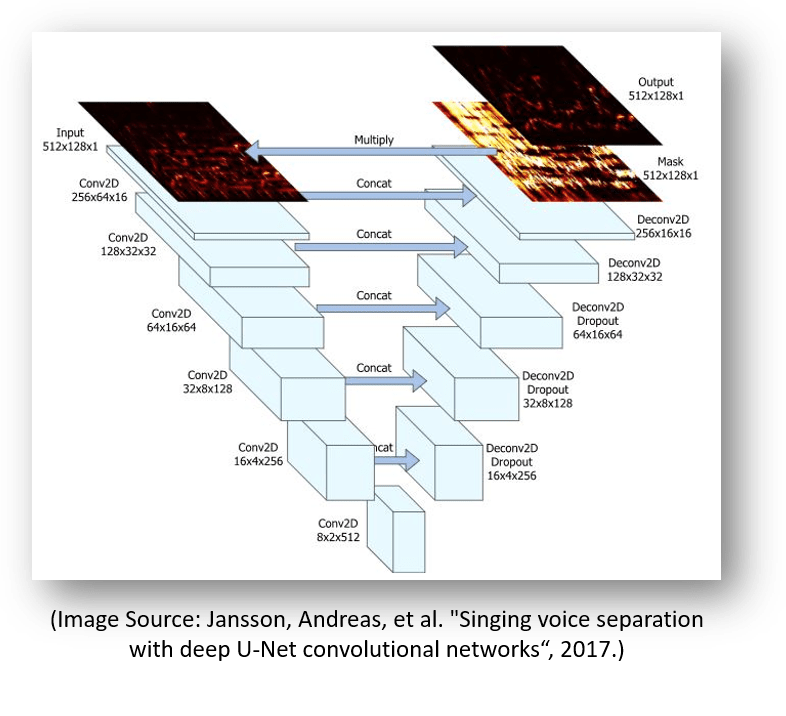
\includegraphics[width=\textwidth]{./figures/chapter02_method/spleeter1.png}
        \caption {Jansson 提出的 deep U-Net convolutional network}
        \label{spleeter1}
    \end{minipage}
    \hfil
\end{figure}

\subsubsection{Demucs}
Demucs~\cite{defossez2019music} FaceBook 基於 wave-u-net~\cite{stoller2018wave} 提出的弱監督訓練模型(圖\ref{demucs1}與圖\ref{demucs2})
\begin{figure}[htbp]
    \hfil
    \begin{minipage}[t]{0.45\textwidth}
        \centering
        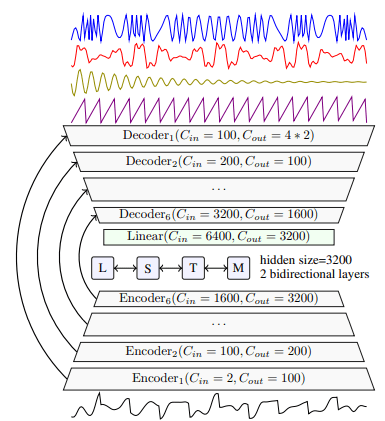
\includegraphics[width=\textwidth]{./figures/chapter02_method/demucs1.png}
        \caption {Demucs 的完整架構}
        \label{demucs1}
    \end{minipage}
    \begin{minipage}[t]{0.45\textwidth}
        \centering
        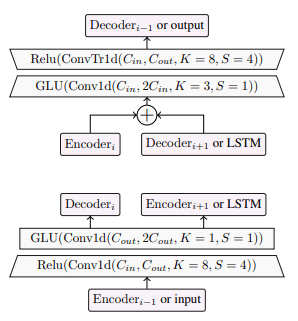
\includegraphics[width=\textwidth]{./figures/chapter02_method/demucs2.png}
        \caption {Encoder 與 decoder 細節}
        \label{demucs2}
    \end{minipage}
    \hfil
\end{figure}
在 wave-u-net 之上,於 encoder 與 decoder 加上了 GLU 的激活函數,也對 biLSTM 增加了更多通道以改進效果。在時域的訊號分離模型中,獲得很大的效能改進,並且也開源其程式碼\footnote{https://github.com/facebookresearch/demucs},對歌聲分離領域有很大的貢獻。

\subsection{注意力模型}
關於注意力模型(attention-based model),必須先談其起源,seq2seq模型的論文自2014年被發表~\cite{vaswani2017attention}以來,使機器在自然語言翻譯領域中取得很好的效果,seq2seq模型基本可以分為兩大部分 encoder 與 decoder,前者會將輸入語句編碼成類向量以表示初始狀態,後者則是使用該類向量預測下一字詞,產生新的文字內容。值得一提的是,輸入給定語句取得翻譯時,並不能觀察期中間產物的向量。

seq2seq模型看似強大,但也有個不可忽視的問題,當模型接受最後一個狀態的語句輸出作為 encoder 的輸入,產生其向量狀態時,RNN模型會有機率忘記太遠的資訊,即使加上LSTM~\cite{gers1999learning}或GLU仍無法妥善解決。此時,注意力模型就起到一個重要的作用,其度量了相似性。若當前的輸入語句與狀態向量越類似,那當前輸入的權重就越大。接下來會以台大李宏毅\footnote{\url{https://speech.ee.ntu.edu.tw/~tlkagk/}}老師的投影片為輔助,稍微解釋機器取得權重的方法(圖\ref{attention-based_model1}),decoder 在計算前會有一組模型參數 $z^0$,會與每個隱狀態 $h^i$ 進行匹配的運算,計算 $z^0$ 與 $h^i$ 的相似度最後得到注意價值度(attention score)$\alpha_0^i$,
\begin{figure}[htbp]
    \hfil
    \begin{minipage}[t]{0.45\textwidth}
        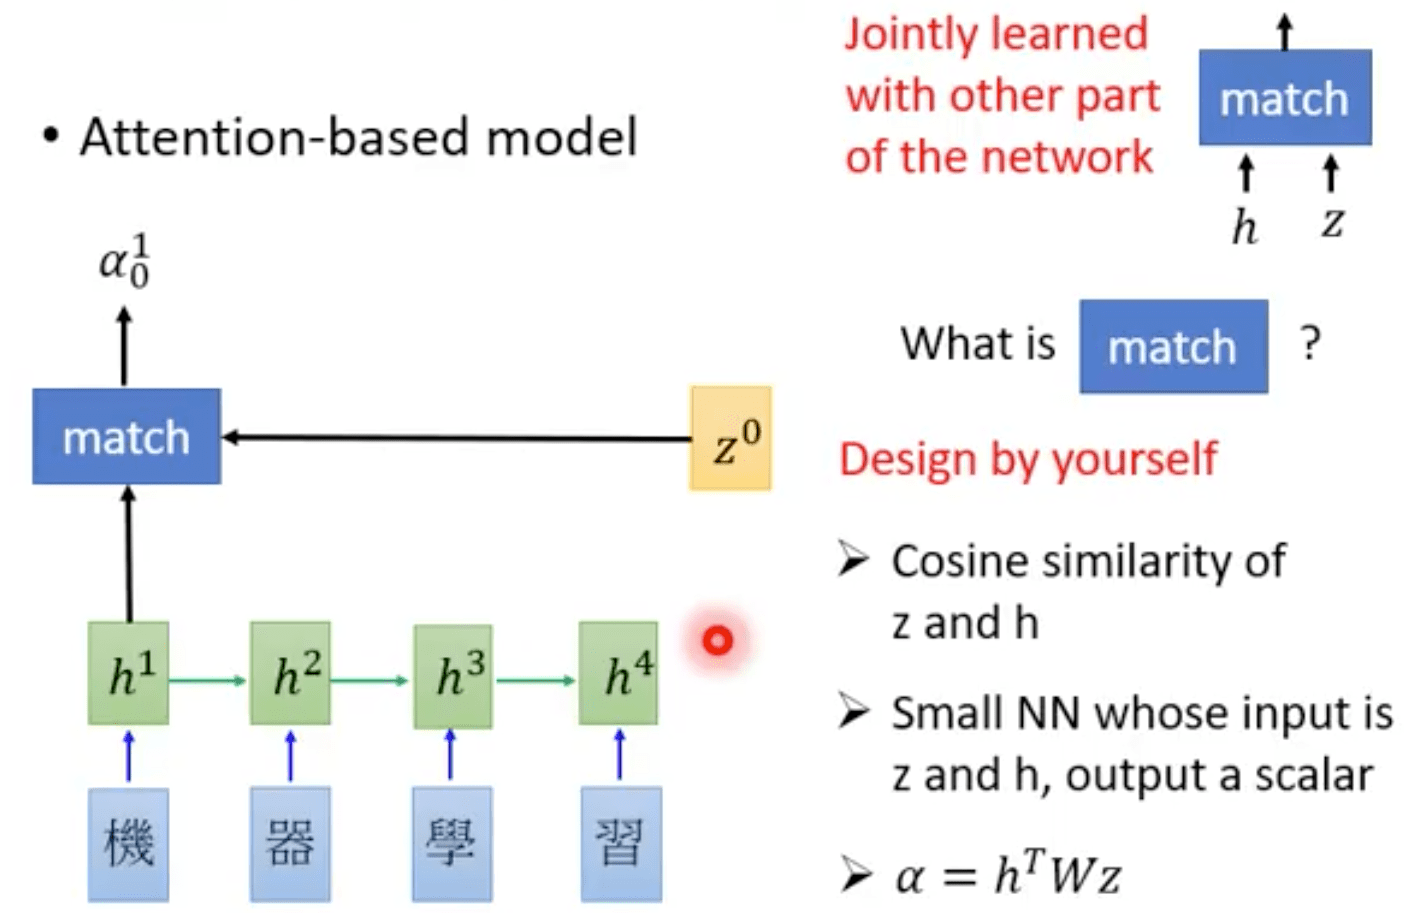
\includegraphics[width=\textwidth]{./figures/chapter02_method/attention-based_model1.png}
        \caption {注意力價值度的計算}
        \label{attention-based_model1}
    \end{minipage}
    \hfil
\end{figure}
得到了 $\alpha_0^i, i\in\{1,2,3,4\}$ 後,取 softmax 轉換成各自機率 $\hat{\alpha}_0^i, i\in\{1,2,3,4\}$,得到注意價值的機率分布,再以此作為隱狀態 $h^i$ 的加權得到 $c^0$(圖\ref{attention-based_model2}),最後給 decoder 進行解碼。 
\begin{figure}[htbp]
    \hfil
    \begin{minipage}[t]{0.45\textwidth}
        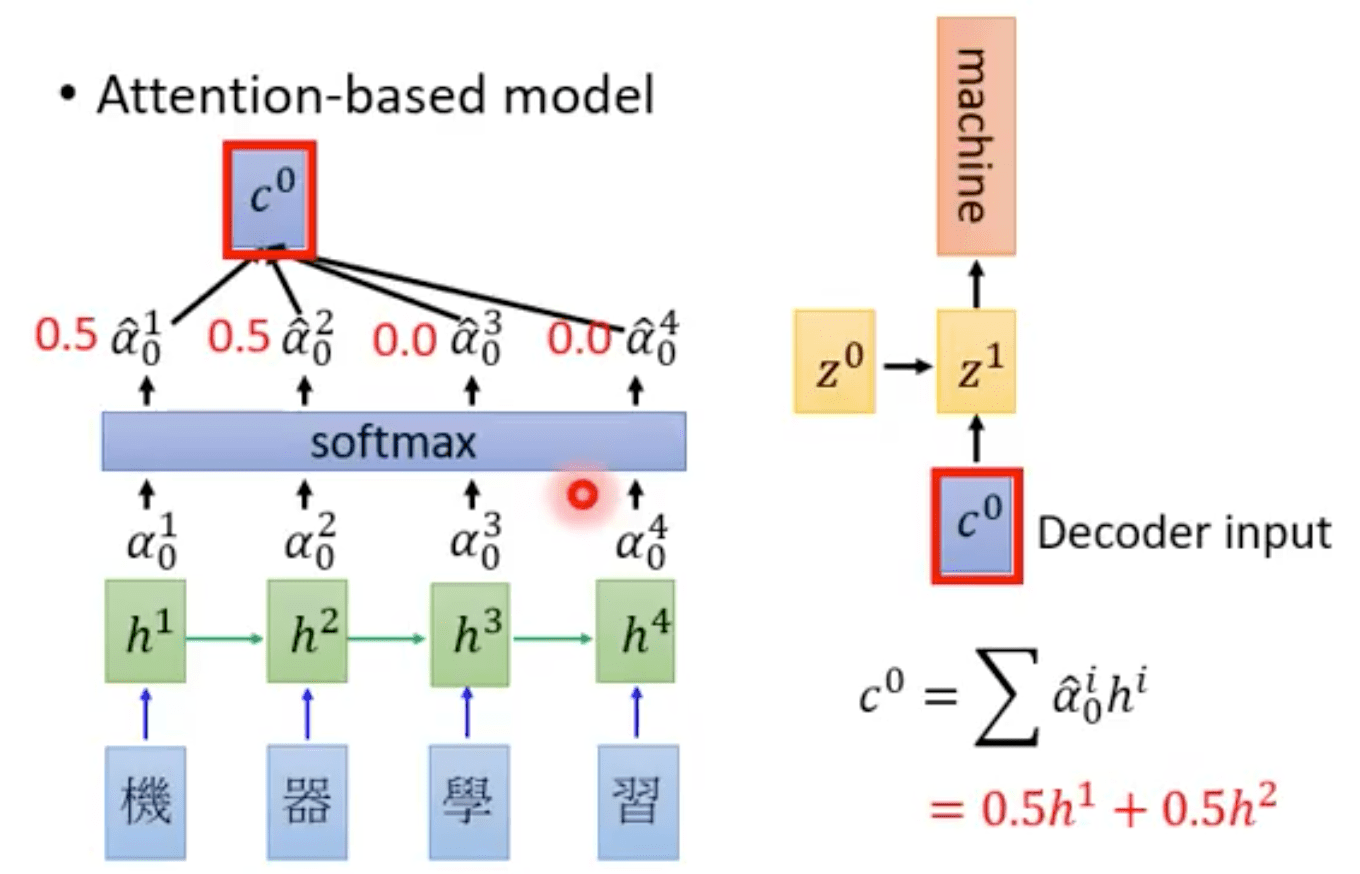
\includegraphics[width=\textwidth]{./figures/chapter02_method/attention-based_model2.png}
        \caption {使用注意力價值度計算新的隱狀態}
        \label{attention-based_model2}
    \end{minipage}
    \hfil
\end{figure}

這邊已經稍微介紹注意力模型的大致做法,接下來會講到其各自不同的實現方法。

\subsubsection{Self-attention}
Y. Liu 等人的研究中~\cite{liu2020voice},將原本在單一維度上使用的 self-attention 改成在雙維度上使用,以利頻譜在 U-Net 上的預測效果,原文指出:相同吉他和弦可能每 10 秒重複一次,對區域性的 CNN filter 來說太長,以致於在 Dense-UNet 中無法抓到這樣的聲音重複資訊;即使使用 BLSTM RNN 進行增強,MMDenseLSTM 仍無法處理跳躍性的聲音重複資訊,因為它只能著重在時間較近的記憶資訊。使用 self-attention 可以注意全局上所有位置的相同序列,並計算區域位置上相同序列的響應值給模型,此方法已經在機器翻譯與圖片生成\footnote{\url{https://github.com/brain-research/self-attention-gan}}領域中獲得採用~\cite{vaswani2017attention,zhang2019self},在改造雙維度上 self-attention 架構上,需要著重頻譜於時間維度上的資訊,期望可以找出音樂訊號中的規律,見圖\ref{self-attention1} 可以看到 self-attention 架構如何應用應用在歌聲分離之上。
\begin{figure}[htbp]
    \hfil
    \begin{minipage}[t]{0.80\textwidth}
        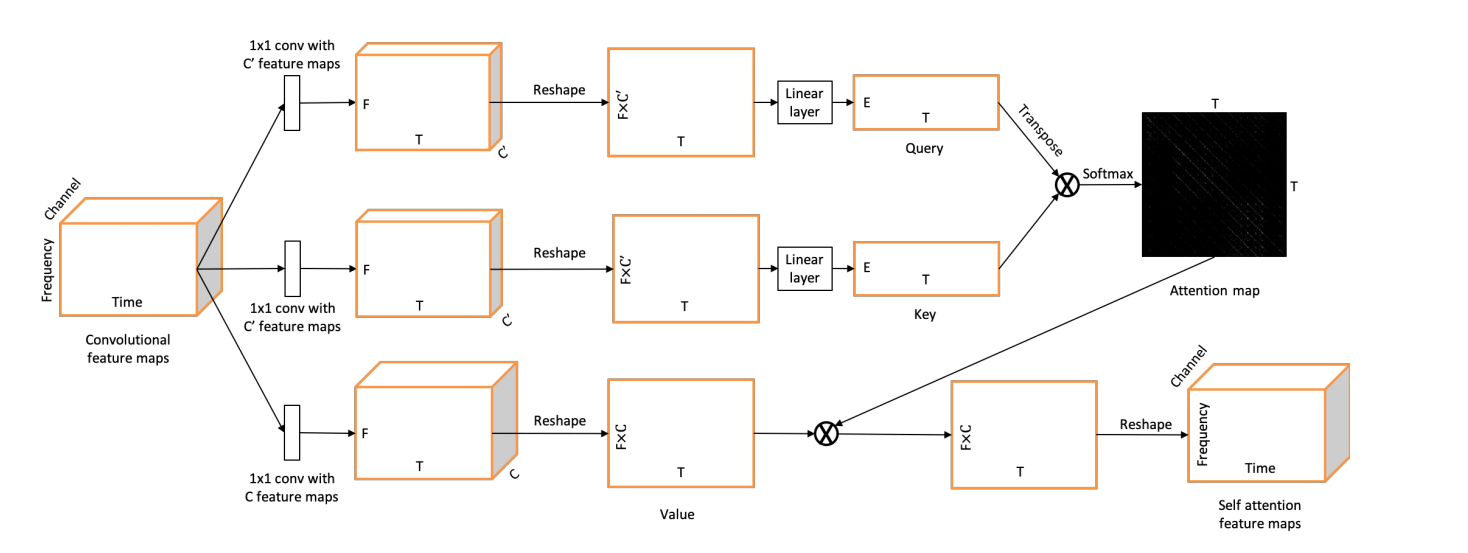
\includegraphics[width=\textwidth]{./figures/chapter02_method/self-attention1.png}
        \caption {Liu 提出的 self-attention 架構}
        \label{self-attention1}
    \end{minipage}
    \hfil
\end{figure}
\begin{figure}[htbp]
    \hfil
    \begin{minipage}[t]{0.80\textwidth}
        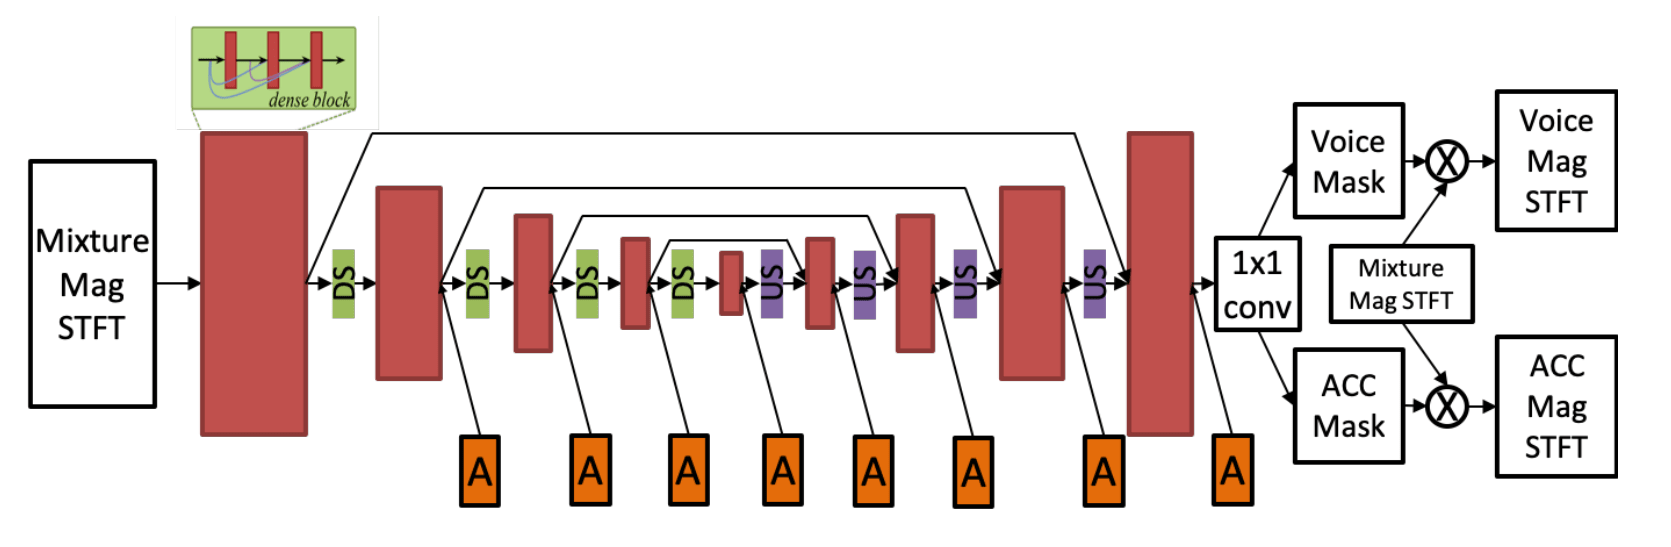
\includegraphics[width=\textwidth]{./figures/chapter02_method/self-attention2.png}
        \caption {Liu 應用在歌聲分離領域的模型架構}
        \label{self-attention2}
    \end{minipage}
    \hfil
\end{figure}

\subsubsection{Attention Gate}
「Attention u-net: Learning where to look for the pancreas」~\cite{oktay2018attention},U-Net 架構本身就很適合執行圖形切割的任務,但若要在醫學領域上可以妥善使用,必須克服少量的訓練資料但又達高精準度。Jetley 等人~\cite{jetley2018learn} 提出了一種 end-to-end\footnote{\url{https://www.itread01.com/content/1546712649.html}} 的 attention 架構「attention gate」,其被常用在自然景照分析與自然語言處理領域中。attention 被使用來彙集分類資訊,使影像分類領域可以更加準確,attention map 可強化有相關的區域,所以可以在各個指標性的資料集中鶴立雞群。
% https://jinglescode.github.io/2019/12/08/biomedical-image-segmentation-u-net-attention/
% https://www.itread01.com/content/1548179294.html#:~:text=%E7%9B%B8%E5%8F%8D%EF%BC%8CHard%20Attention%E6%98%AF%E4%B8%80%E5%80%8B,%E4%BC%B0%E8%A8%88%E6%A8%A1%E7%B5%84%E7%9A%84%E6%A2%AF%E5%BA%A6%E3%80%82
% https://kknews.cc/zh-tw/tech/ql559ao.html

Khened~\cite{khened2019fully} 與 Roth~\cite{roth2018spatial} 等人為了提升影像分割領域效能,需要倚靠額外的區域物件偵測模型隨後幫助圖形分割,研究後發現,在 U-Net 加上 attention gate 可以有效完成這件事,且不增加太多運算時間。在 U-Net 的並接運算(concatenation)之前,先合成全域有相關的激活值,這就是 attention gate (圖\ref{attention_gate1})的實現過程。
\begin{figure}[htbp]
    \hfil
    \begin{minipage}[t]{0.8\textwidth}
        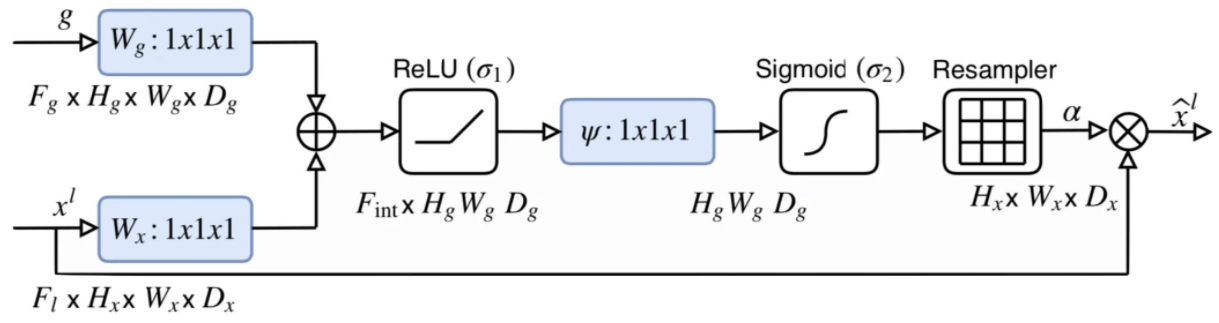
\includegraphics[width=\textwidth]{./figures/chapter02_method/attention_gate1.png}
        \caption {attention gate 架構}
        \label{attention_gate1}
    \end{minipage}
    \hfil
\end{figure}


\section{模型壓縮方法}
% 模型壓縮的東西~\cite{buciluǎ2006model}
雖然目前的硬體設備隨著摩爾定律越來越強,但人們也對低功耗的需求也與日俱增,套用在端點裝置如:手機、工廠監控晶片或是配置低的筆記型電腦。模型剪枝不只探討縮小也研究更快的執行,可以在實時的狀態下使用,如此一來可以更加貼近人們的生活。
% https://zhuanlan.zhihu.com/p/138059904


\subsection{模型剪枝}
本節探討模型剪枝(model pruning),模型壓縮的一種方法。下文探討的 MobileNets~\cite{howard2017mobilenets} ,其模型著重在圖形辨識領域之上,將傳統的卷積神經網路(CNN)改造,使之運算量大幅下降,這雖將模型裡訓練的參數大幅降低,可能導致效果便差,但既有 U-Net 足夠複雜的情況下,經過調整是有妥協空間的,接下來的子節會一一加以探討。

\subsubsection{深度可分卷積}
深度可分卷積(depth-wise separable convolution)是一種對普通卷積參數削減的方法,在 Chollet~\cite{chollet2017xception} 等人所提出的 xception 使用後被廣為人知,其採用深度可分卷積替換 inception v3 中的普通卷積,原作者的初衷是使 inception v3 架構更寬,但又不讓網路參數提升。Google 於 2017 提出的 MobileNet~\cite{howard2017mobilenets} 模型,欲解決巨大網路模型的瓶頸—卷積,在不降太多效能的情況下,使用深度可分卷積盡量減少原始卷積的計算量,將模型可以套用在手機或是攜帶裝置之上。

探討深度可分卷積與一般卷積的差異,運算量是非常值得關注的,為了方便解說,先定義一些使用到的參數:
\begin{itemize}
    \item 輸入資料 $F$
    \subitem 長 $=$ 寬 $=D_F$;高 $=M$
    \item 輸出資料 $G$
    \subitem 長 $=$ 寬 $=D_G$;高 $=N$
    \item 卷積 Kernel $K$
    \subitem 長 $=$ 寬 $=D_K$;高 $=M$;卷積數量 $=N$
    \subitem 卷積大小 $D_K \times D_K \times M \times N$
\end{itemize}
普通卷積在計算計算輸出資料 $G$ 的情況:
\begin{itemize}
    \item $G_{k,l,n}=\sum_{i,j,m}K_{i,j,m}\cdot F_{k+i-1,l+j-1,m}$
    \item 總運算量 $D_K \times D_K \times M \times N \times D_F \times D_F$
\end{itemize}
深度可分卷積在計算輸出資料 $\hat{G}$ 的情況:
\begin{itemize}
    \item $\hat{G}_{k,l,n}=\sum_{i,j}\hat{K}_{i,j,m}\cdot F_{k+i-1,l+j-1,m}$
    \item 總運算量 $D_K \times D_K \times M \times D_F \times D_F + M \times N \times D_F \times D_F$
\end{itemize}
其減少的運算量:
\begin{equation*}
\begin{split}
    \frac{\textup{Depthwise Separable Conv.}}{\textup{Normal Conv.}} \\
    = \frac{D_K \times D_K \times M \times D_F \times D_F + M \times N \times D_F \times D_F}{D_K \times D_K \times M \times N \times D_F \times D_F} \\
    = \frac{1}{N} + \frac{1}{D_K^2} &
\end{split}
\end{equation*}

舉例來說\footnote{\url{https://towardsdatascience.com/a-basic-introduction-to-separable-convolutions-b99ec3102728}
},輸入為一個$12\times 12\times 3$的圖,使用一個 $5\times5$ 二維卷積(no padding 與 1 stride),input(12x12) $\rightarrow$ conv(5x5) $\rightarrow$ output(8x8),普通卷積需要 1228800  運算量(圖\ref{depthwise_separable_conv1});深度可分卷積需要 53952 運算量(圖\ref{depthwise_separable_conv2})。縮小比值:0.043。

\begin{figure}[htbp]
    \hfil
    \begin{minipage}[t]{0.60\textwidth}
        \centering
        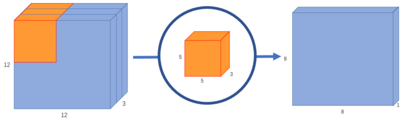
\includegraphics[width=\textwidth]{./figures/chapter02_method/depthwise_separable_conv1.png}
    \end{minipage}
    \caption {普通卷積的運算:需要 $256\times((3\times5\times5)\times(8\times8))=1228800$ 運算量}
    \label{depthwise_separable_conv1}
    \hfil
\end{figure}

\begin{figure}[htbp]
    \hfil
    \begin{minipage}[t]{1.0\textwidth}
        \centering
        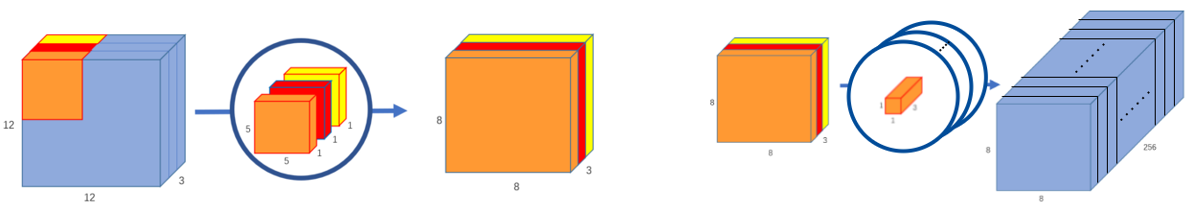
\includegraphics[width=\textwidth]{./figures/chapter02_method/depthwise_separable_conv2.png}
        \caption {深度可分卷積的運算:需要 $(3\times5\times5)\times(8\times8)+256\times((3\times1\times1)\times(8\times8))=53952$ 運算量}
        \label{depthwise_separable_conv2}
    \end{minipage}
    \hfil
\end{figure}


\subsubsection{Inverted Residuals 與 Linear Bottlenecks}
在訓練卷積神經網路模型時,比如本論文探討的 U-Net baseline,經常是層層堆疊,且對於每層的輸出,為了保留其最有用的資訊「manifold of interest」,會將其嵌入至一個低維度的子空間進行訓練。針對深度可分卷積架構,要如何在輕量化網路參數又不喪失太多資訊,MobileNet V2~\cite{sandler2018mobilenetv2} 提出的做法(圖\ref{inverted_residuals1}):
\begin{itemize}
    \item[1.] 作 depthwise separable convolution 前,先作一層 pointwise convolution 提升輸出維度(此作法稱為「linear bottleneck layer」)
    \item[2.] 最後輸出前使用「linear activation function」以避免過度的資訊過濾
\end{itemize}
\begin{figure}[htbp]
    \hfil
    \begin{minipage}[t]{0.65\textwidth}
        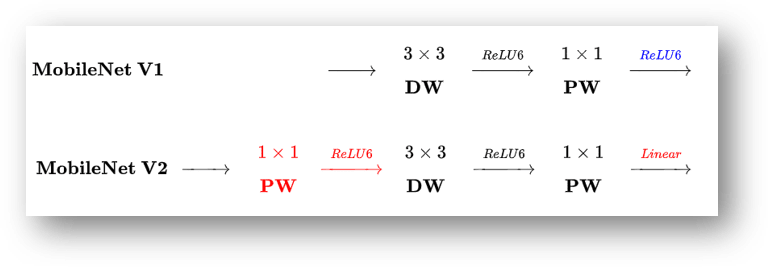
\includegraphics[width=\textwidth]{./figures/chapter02_method/inverted_residuals1.png}
        \caption {MobileNet V2 對深度可分卷積做出的改進}
        \label{inverted_residuals1}
    \end{minipage}
    \hfil
\end{figure}
而如此的作法極相似於 Resnet~\cite{he2016deep} 中被廣泛使用的 residual block,(圖\ref{inverted_residuals2}-(a))在過去會將 channel 先壓縮在進行卷積, shortcut 連接兩個較大的 channel 以傳遞資訊,(圖\ref{inverted_residuals2}-(b))在 MobileNet V2 中,shortcut 連接兩個較小的 channel,是為了將經過「linear bottleneck layer」中有用的資訊「manifold of interest」嵌入至低維度的子空間。
\begin{figure}[htbp]
    \hfil
    \begin{minipage}[t]{0.65\textwidth}
        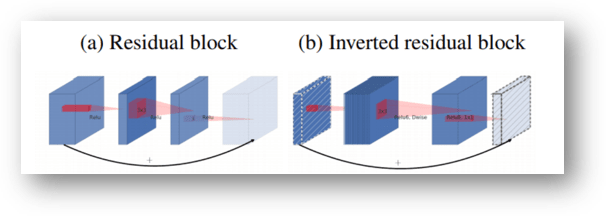
\includegraphics[width=\textwidth]{./figures/chapter02_method/inverted_residuals2.png}
        \caption {Inverted residuals}
        \label{inverted_residuals2}
    \end{minipage}
    \hfil
\end{figure}


\subsection{模型量化}
模型量化由模型與量化兩詞組成。在深度學習領域下,模型指的是神經網路。而量化是指降低精準度,通常以定點(通常為「int8」)近似浮點數模型,從而降低模型儲存於記憶體的消耗,也有機會可以加速模型在預測的速度,下式與圖 表示基本的線性量化方法。

\begin{itemize}
    \item 量化(Quantize)
    \subitem $x_\textup{int} = \textup{round}(\frac{x}{\Delta})+z$
    \subitem $x_Q = \textup{clamp}(0,N_\textup{levels}-1,x_\textup{int})$
    \item 反量化(De-quantize)
    \subitem $x_\textup{float} = (x_Q-z)\times\Delta$
\end{itemize}
\begin{figure}[htbp]
    \hfil
    \begin{minipage}[t]{0.4\textwidth}
        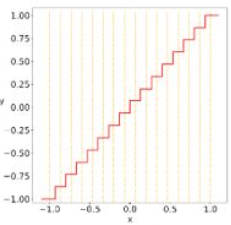
\includegraphics[width=\textwidth]{./figures/chapter02_method/quantization1.png}
        \caption {基礎線性量化}
        \label{quantization1}
    \end{minipage}
    \hfil
\end{figure}

\subsubsection{Quantized Neural Networks PACKage}
QNNPACK (quantized neural networks package)~\cite{dukhan2018qnnpack,wu2019machine} 是 Marat Dukhan 開發專用於量化神經網路計算的 Python 套件,其卓越的性能,在2019年一經開源\footnote{\url{https://github.com/pytorch/QNNPACK}}就擊敗了幾乎當時全部已公開的加速演算法。接下來本節會參考此\footnote{\url{https://jackwish.net/2019/reveal-qnnpack-implementation.html}}文章以描述 QNNPACK 的實現方法。在矩陣乘法優化階段,是針對輸出矩陣的劃分,拆分成圖\ref{qnnpack1} 的 $MR \times NR$ 小塊,再做矩陣的乘法,提高指令集的使用度。
\begin{figure}[htbp]
    \hfil
    \begin{minipage}[t]{0.8\textwidth}
        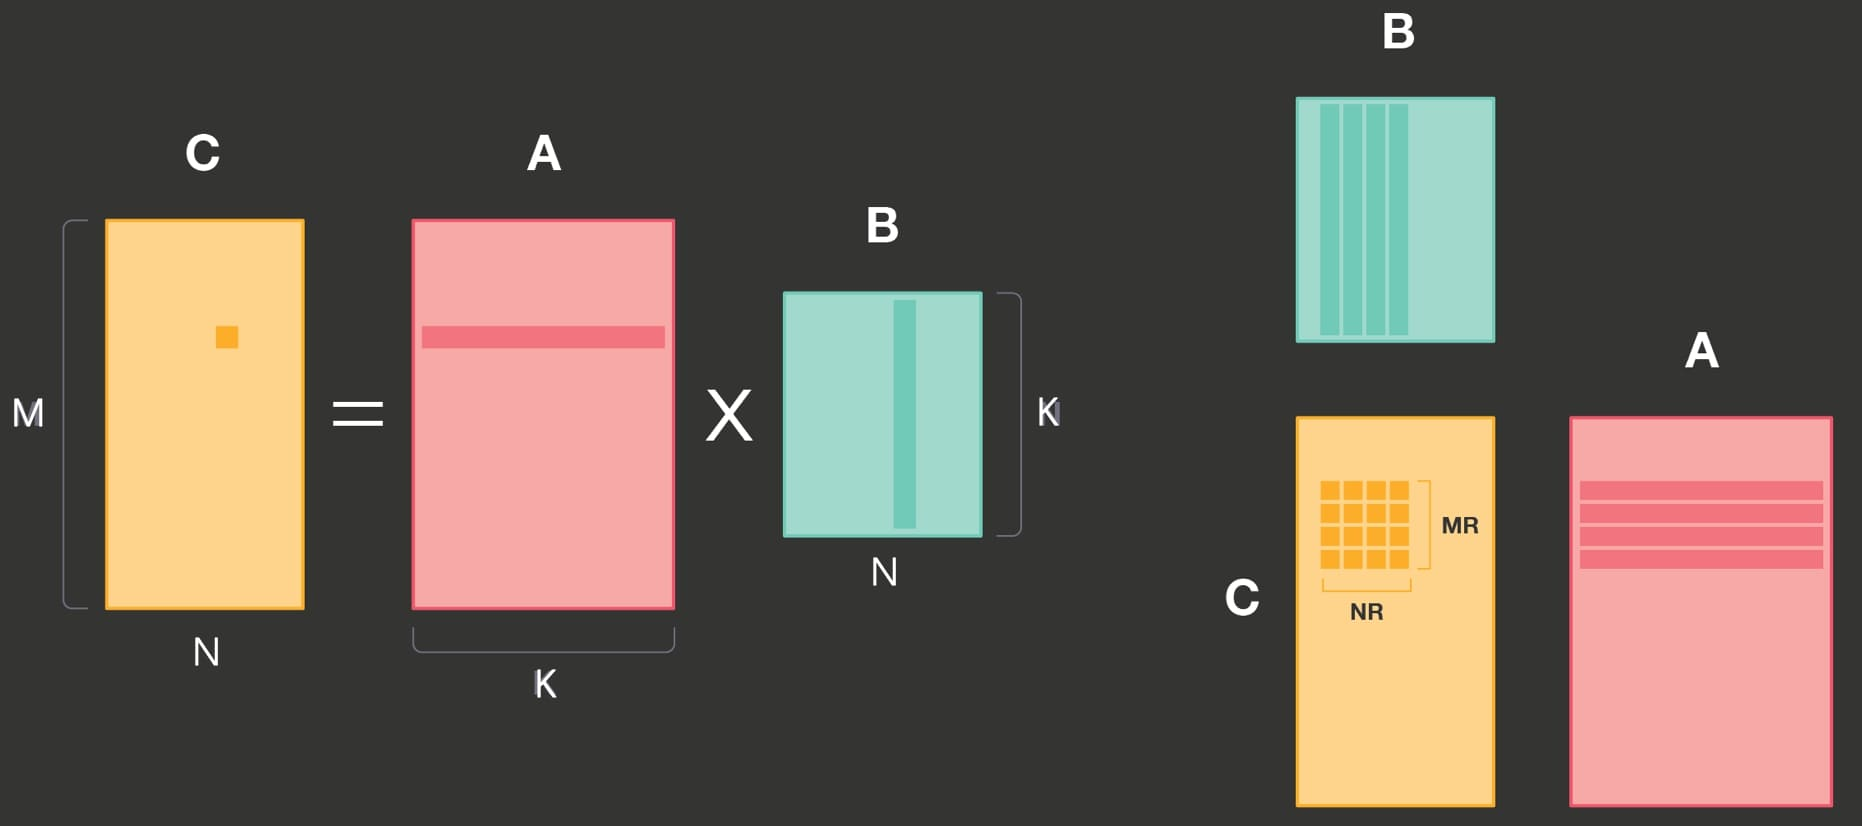
\includegraphics[width=\textwidth]{./figures/chapter02_method/qnnpack1.jpg}
        \caption {QNNPACK 的矩陣乘法優化}
        \label{qnnpack1}
    \end{minipage}
    \hfil
\end{figure}
矩陣乘法的優化中,QNNPACK 也改變實現矩陣乘法的底層以提高了 armv7 與 arm64 指令集的使用度,計算過程妥善使用 L1 cache 的優勢,亦對記憶體進行重新組織(repacking),以改進高速緩存的命中率。